\section{Theoretical Analysis}
\label{sec:analysis}

In this section, the circuit shown in Figure~\ref{fig:Circuit_Base} is analyzed theoretically with the Nodal Method and General Solution Method in order to caracterize it in the interval $\left[-5,20\right[$.

\subsection{Step 1: Solution for $t<0$}

When $t<0$ we consider that the circuit is in equilibrium and, because of that, no current passes through the capacitor, since the relation between current and voltage in this component is:
\begin{equation}
  \frec{dV}{dt}=\frac{I}{C} \rightarrow I = 0.
  \label{eq:Cap}
\end{equation}

Hence, we can simplify the circuit:
\begin{figure}[h] \centering
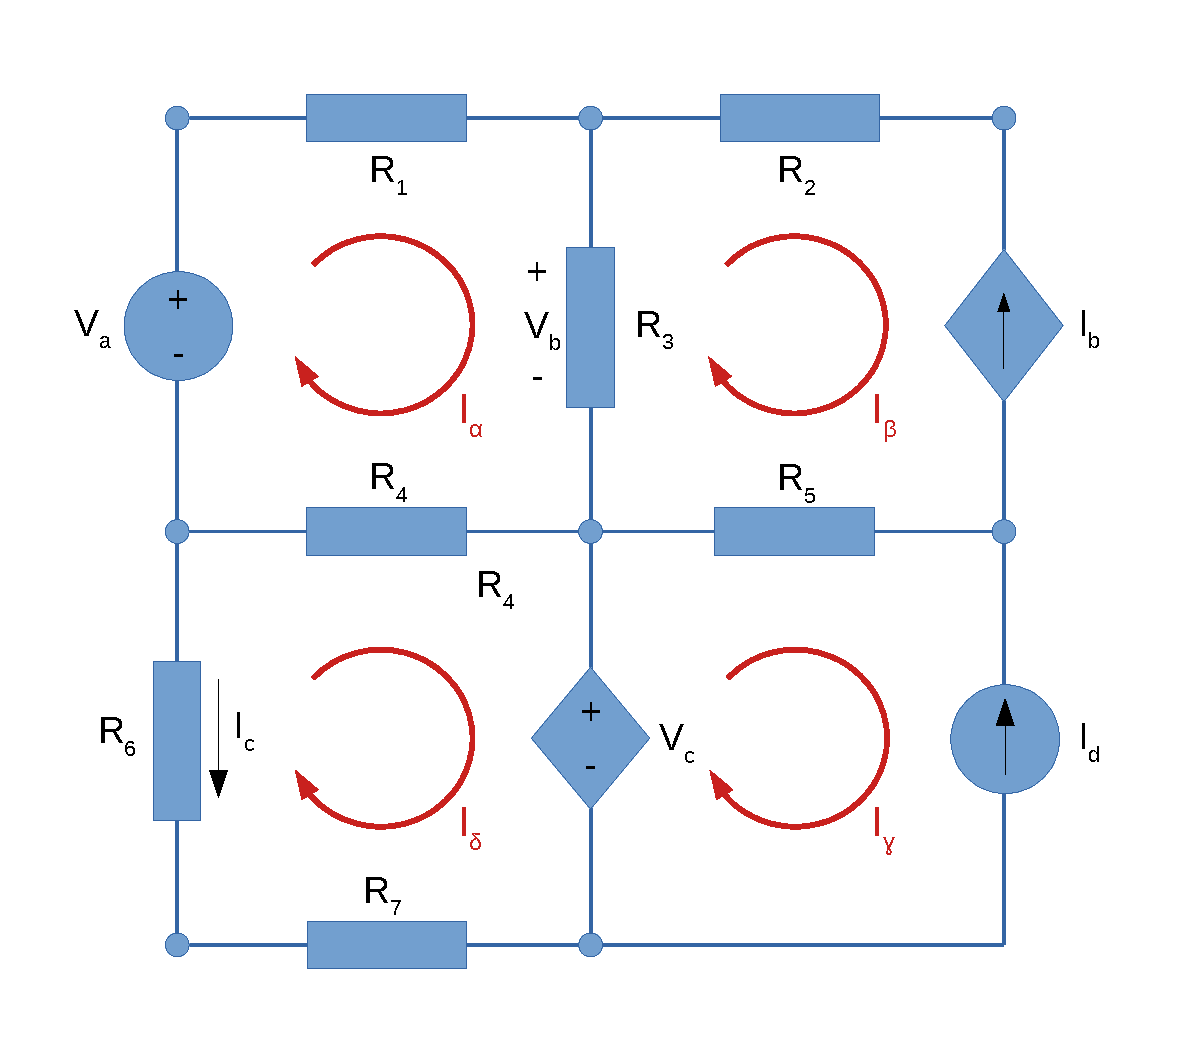
\includegraphics[width=0.45\linewidth]{CircuitMesh.pdf}
\caption{Circuit analysed with mesh currents.}
\label{fig:Circuit_Passo1}
\end{figure}

Applying the Nodal Method to this circuit leads to the following equations:

\begin{equation}
\begin{cases}
	v_1 - v_4 &= V_s;																				  \\
	\frac{1}{R_1}v_1 - (\frac{1}{R_2}+\frac{1}{R_1}+\frac{1}{R_3})v_2 + (\frac{1}{R_2})v_3 + \frac{1}{R_3}v_5 &= 0; 																						  \\
  	\frac{1}{R_2}v_2 - \frac{1}{R_2}v_3+ I_b &= 0;													  \\
  	-\frac{1}{R_1}v_1 + \frac{1}{R_1}v_2 - (\frac{1}{R_4}+\frac{1}{R_6})v_4 + \frac{1}{R_4}v_5 + \frac{1}{R_6}v_7 &= 0;			  																	  \\
	v_5 - v_8 - V_d &= 0;																			  \\
  	\frac{1}{R_5}v_5 - \frac{1}{R_5}v_6 - I_b &= 0;												  	  \\
  	-(\frac{1}{R_7}+\frac{1}{R_6})v_7 + \frac{1}{R_7}v_8 + \frac{1}{R_6}v_4 &= 0;					  \\
	v_2 - v_3 - V_b &= 0;																			  \\
  	\frac{1}{R_6}v_4 - \frac{1}{R_6}v_7 - I_d &= 0;													  \\
  	v_4 &= 0;																						  \\
  	-K_bV_b + I_b &= 0;																				  \\
  	V_d - K_cI_c &= 0.
\end{cases}
\end{equation}

Where the $2^{nd}$, $3^{rd}$, $6^{th}$ and $7^{th}$ are the equations in the respective nodes; the $1^{st}$ and $5^{th}$ are the relations imposed by the voltages soureces in those nodes; the $4^{th}$ is the supernode that bypasses $V_s$; the $8^{th}$ to $10^{th}$ are the relations between the circuit and, in order, $V_b$, $I_d$ and $v_4$; the final two equations are the ones that describe $I_b$ and $V_d$, respectivly. 
The solution to this linear system of equations is determined by Octave, plus the currents flowing in the circuit using Ohm's Law to the resistor's branches and Kirchhoff Current Law~(KCL) to the branches with voltage sources:

\begin{table}[h]
  \centering
  \begin{tabular}{|l|r|}
    \hline    
    {\bf Name} & {\bf Value [A or V]} \\ \hline
    \input{../mat/PASSO1_tab}
  \end{tabular}
  \caption{Variables in the Mesh Method. A variable preceded by @ is of type {\em current} and expressed in Ampere; other variables are of type {\em voltage} and expressed in Volt.}
  \label{tab:PASSO1}
\end{table}

All the currents were measured from the lower numbered node to the higher one; so, the direction of the current that passes through $R_6$ is, if the result is positive, from $v_4$ to $v_7$.

\subsection{Step 2: Solution for $t=0$ and $R_{eq}$}

Once found the solution for the nodes in $t<0$, the next step is to calculate the boundary conditions for the knots in the circuit, because the voltage in the nodes doesn't necessarily need to be continuos, only the difference of potencial in the capacitor, $V_c$. Therefor, a non continuos change in a power source, in this case in the voltage source $V_s$, might lead to a diferent voltage in the nodes.
Since the solution to this circuit will also be divided in natural and forced, we can use this step to evaluate the equivelent resistance of the circuit, $R_{eq}$.

To evaluate the circuit at $t=0$, we must have in mind that $V_c$ is continuos, so $V_c(0)=V_c(0^-)$. Another point to take into account is that, for the natural solution, we can ignore the sinusoidal part of $V_s$, which leaves us with $V_s=0$. In this conditions, we can say that the circuit~\ref{fig:Circuit_Base} is identical to this one:

\begin{figure}[h] \centering
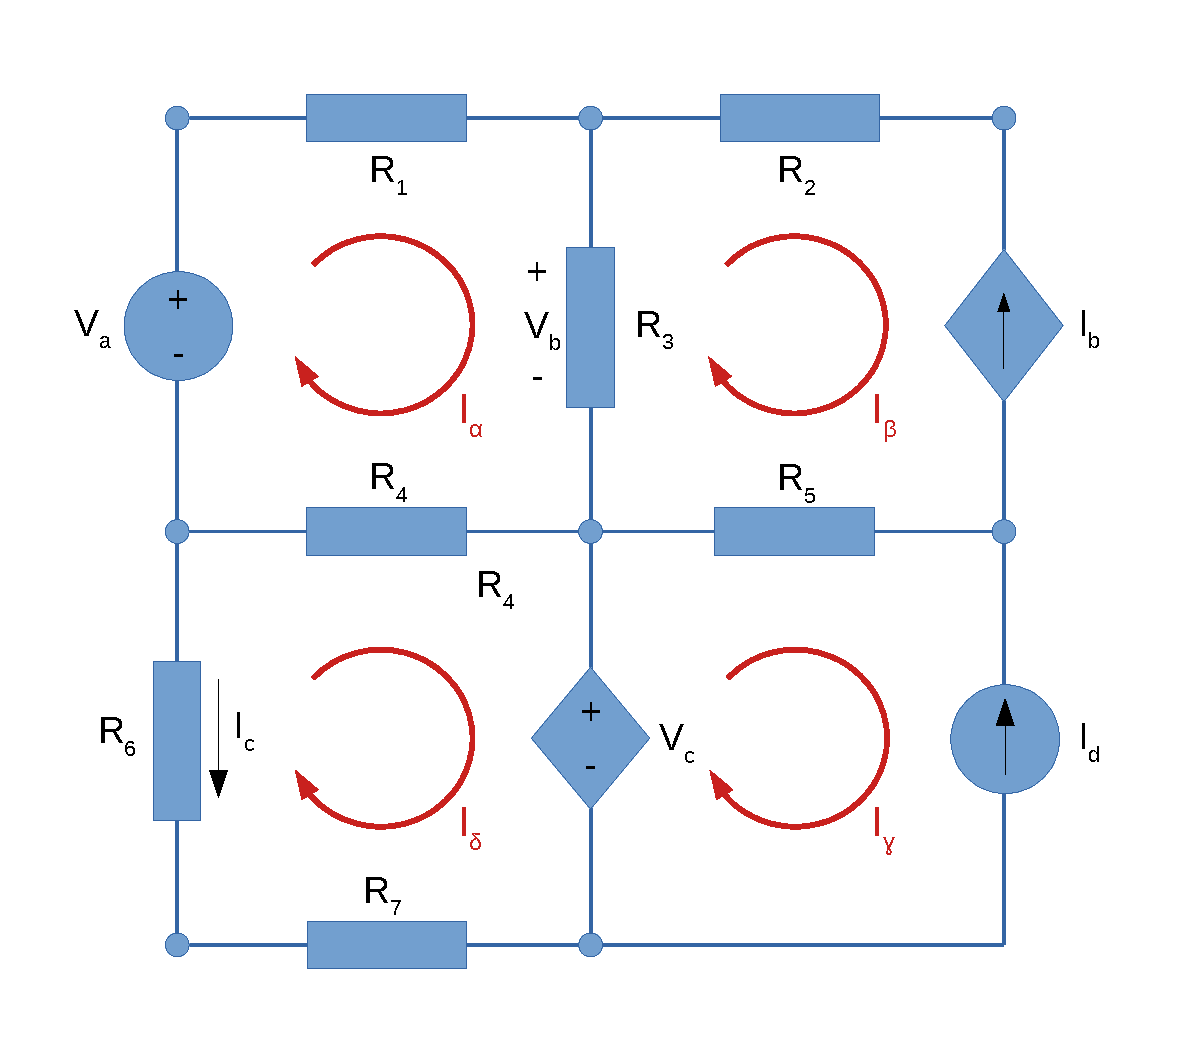
\includegraphics[width=0.45\linewidth]{CircuitMesh.pdf}
\caption{Circuit analysed with mesh currents.}
\label{fig:Circuit_Passo2}
\end{figure}

The set of equations that describe it are, using the Nodal Method:

\begin{equation}
\begin{cases}
	v_1 - v_4 &= 0;																				  	  \\
	\frac{1}{R_1}v_1 - (\frac{1}{R_2}+\frac{1}{R_1}+\frac{1}{R_3})v_2 + (\frac{1}{R_2})v_3 + \frac{1}{R_3}v_5 &= 0; \\
  	\frac{1}{R_2}v_2 - \frac{1}{R_2}v_3+ I_b &= 0;													  \\
  	-\frac{1}{R_1}v_1 + \frac{1}{R_1}v_2 - (\frac{1}{R_4}+\frac{1}{R_6})v_4 + \frac{1}{R_4}v_5 + \frac{1}{R_6}v_7 &= 0;			  																	  \\
	v_5 - v_8 - V_d &= 0;																			  \\
  	v_6 - v_8 - V_c &= 0;											  	  							  \\
  	-(\frac{1}{R_7}+\frac{1}{R_6})v_7 + \frac{1}{R_7}v_8 + \frac{1}{R_6}v_4 &= 0;					  \\
	v_2 - v_3 - V_b &= 0;																			  \\
  	\frac{1}{R_6}v_4 - \frac{1}{R_6}v_7 - I_d &= 0;													  \\
  	v_4 &= 0;																						  \\
  	-K_bV_b + I_b &= 0;																				  \\
  	V_d - K_cI_c &= 0.
\end{cases}
\end{equation}

Where the $2^{nd}$, $3^{rd}$ and $7^{th}$ are the equations in the respective nodes; the $1^{st}$, $5^{th}$ and $6^{th}$ are the relations imposed by the voltages soureces in those nodes; the $4^{th}$ is the supernode that bypasses $V_s$; the $8^{th}$ to $10^{th}$ are the relations between the circuit and, in order, $V_b$, $I_d$ and $v_4$; the final two equations are the ones that describe $I_b$ and $V_d$, respectivly. 
We note that 
\begin{equation}
	I_c = I_b + \frac{v_6-v_5}{R_5},
\end{equation}
\begin{equation}
	R_{eq} = \frac{V_c}{I_c}, \text{ and}
\end{equation}
\begin{equation}
	\tau = R_{eq}C.
\end{equation}


The solution to this linear system of equations is determined by Octave, plus the currents flowing in the circuit using Ohm's Law to the resistor's branches and Kirchhoff Current Law~(KCL) to the branches with voltage sources:

\begin{table}[h]
  \centering
  \begin{tabular}{|l|r|}
    \hline    
    {\bf Name} & {\bf Value [A or V]} \\ \hline
    \input{../mat/PASSO2_tab}
  \end{tabular}
  \caption{Variables in the Mesh Method. A variable preceded by @ is of type {\em current} and expressed in Ampere; other variables are of type {\em voltage} and expressed in Volt.}
  \label{tab:PASSO2}
\end{table}


\subsection{Step 3: Natural Solution for $t>0$}

Using $R_{eq}$ and $v_6$ from the previous step we can compute the natural solution of $v_6(t)$:

\begin{equation}
	
	v_6(t) =& v_6(+\infty) - (v_6(+\infty) - v_6(0))e^{-\frac[1}[\tau}t}		\\
	v_6(t) =& v_6(0))e^{-\frac[1}[\tau}t}, \text{ dado que } (v_6(+\infty) = 0.
	
\end{equation}

Using Octave to plot this equation gives us:

\begin{figure}[h] \centering
\includegraphics[width=0.45\linewidth]{../mat/PASSO3.eps}
\caption{Natural solution of $v_6(t)$.}
\label{fig:TEO_NAT_SOL}
\end{figure}

\subsection{Step 4: Forced Solution for $t>0$}

Since $V_s$ is a sinusoidal source in $t>0$, we can perform a complex analysis, replacing all the componets for their impedances. In this case, only the capacitor changes (since all resistors have the same impedance):

\begin{equation}
	
	Z_c = \frac{j\omegaC}
	
\end{equation}

Where $\omega$ is the frequency ($1k rads^{-1}$).
Saying that $V_s = 1$ to calculate the phasors relative to $V_s$ and using the Nodal Method we arive to a set of equations:

\begin{equation}
\begin{cases}
	v_1 - v_4 &= 1;																				  	  \\
	\frac{1}{R_1}v_1 - (\frac{1}{R_2}+\frac{1}{R_1}+\frac{1}{R_3})v_2 + (\frac{1}{R_2})v_3 + \frac{1}{R_3}v_5 &= 0; \\
  	\frac{1}{R_2}v_2 - \frac{1}{R_2}v_3+ I_b &= 0;													  \\
  	-\frac{1}{R_1}v_1 + \frac{1}{R_1}v_2 - (\frac{1}{R_4}+\frac{1}{R_6})v_4 + \frac{1}{R_4}v_5 + \frac{1}{R_6}v_7 &= 0;			  																	  \\
	v_5 - v_8 - V_d &= 0;																			  \\
  	\frac{1}{R_5}v_5 - (\frac{1}{R_5} + j\omegaC)v_6 + (j\omegaC)v_8- I_b &= 0;						  \\
  	-(\frac{1}{R_7}+\frac{1}{R_6})v_7 + \frac{1}{R_7}v_8 + \frac{1}{R_6}v_4 &= 0;					  \\
	v_2 - v_3 - V_b &= 0;																			  \\
  	\frac{1}{R_6}v_4 - \frac{1}{R_6}v_7 - I_d &= 0;													  \\
  	v_4 &= 0;																						  \\
  	-K_bV_b + I_b &= 0;																				  \\
  	V_d - K_cI_c &= 0.
\end{cases}
\label{eq:PASSO4}
\end{equation}

Where the $2^{nd}$, $3^{rd}$, $6^{th}$ and $7^{th}$ are the equations in the respective nodes; the $1^{st}$ and $5^{th}$ are the relations imposed by the voltages soureces in those nodes; the $4^{th}$ is the supernode that bypasses $V_s$; the $8^{th}$ to $10^{th}$ are the relations between the circuit and, in order, $V_b$, $I_d$ and $v_4$; the final two equations are the ones that describe $I_b$ and $V_d$, respectivly. 

The solution to this linear system of equations is determined by Octave:

\begin{table}[h]
  \centering
  \begin{tabular}{|l|r|}
    \hline    
    {\bf Name} & {\bf Value} \\ \hline
    \input{../mat/PASSO4_tab}
  \end{tabular}
  \caption{Variables in the Nodal Method. Variables are adimentional.}
  \label{tab:PASSO4}
\end{table}

The forced solution of $v_6(t)$ is given by $v_6(t) = V_s(t)*Pv_6$.

\subsection{Step 5: Total Solution for $t\in [-5,20]ms$}

The total solution of $v_6$ will be the solution from step 1 for $t\in [-5,0[ms$ and the sum of the natural solution and forced solution for $t\in [0,20]ms$
The plot given by Octave is:

\begin{figure}[h] \centering
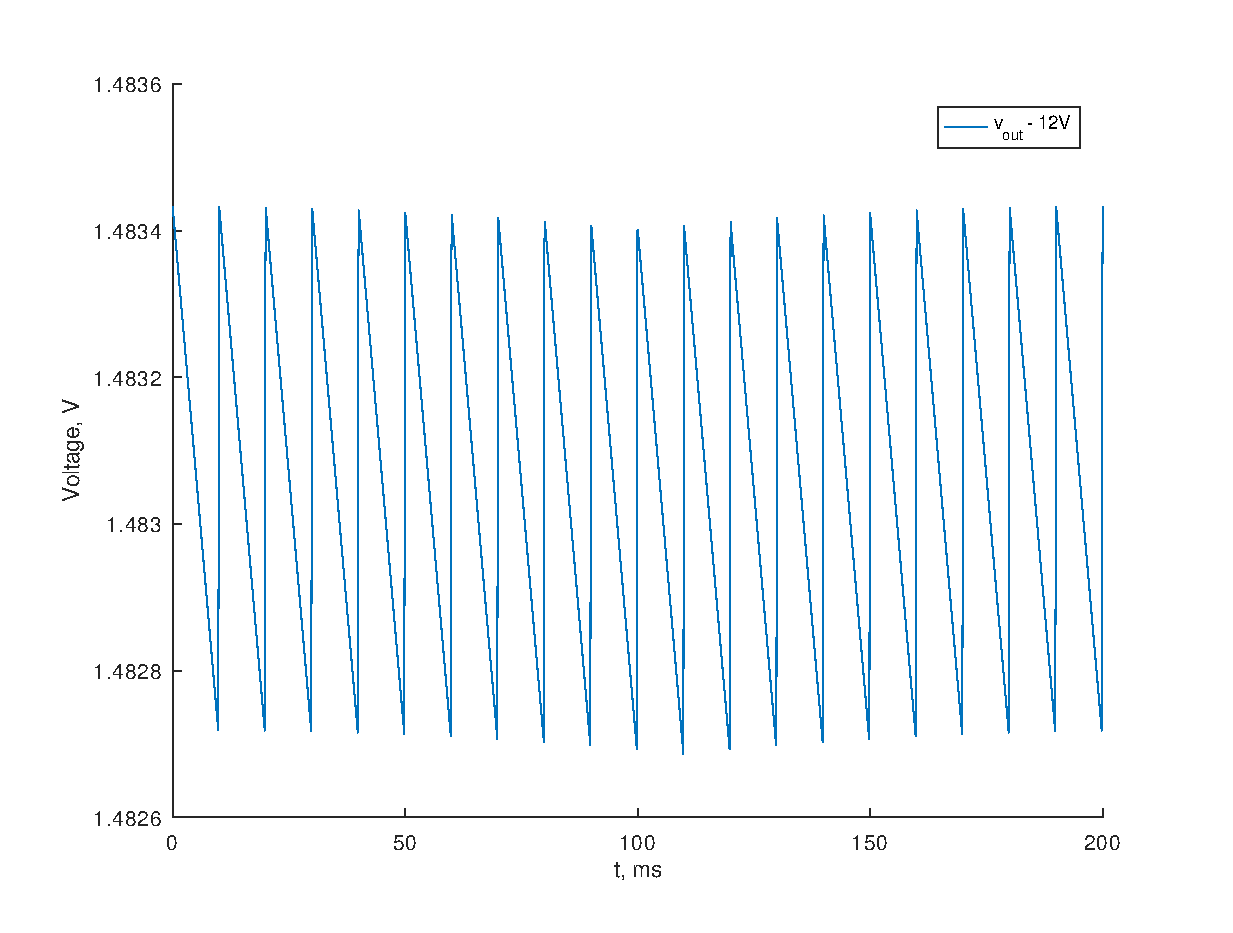
\includegraphics[width=0.45\linewidth]{../mat/PASSO5.eps}
\caption{Total solution of $v_6(t)$ and $V_s(t)$.}
\label{fig:TEO_TOT_SOL}
\end{figure}

\subsection{Step 6: Frequency Response of $v_6$ and $V_c$}

In this subsection is made an analysis of the frequency response of $v_6$ and $V_c$ in order to $V_s$. for that we need to solve the same system as in step 4 (equation \ref{eq:PASSO4}), with $\omega$ as a parameter. The magnitude (absolute value of the complex vectors) and phase (angle of the complex vectors is ploted using Octave:

\begin{figure}[h] \centering
\includegraphics[width=0.45\linewidth]{../mat/PASSO6-AMPLITUDE.eps}
\caption{Magnitude responce of $V_s$, $v_6(t)$, $V_c(t)$ and $v_8$.}
\label{fig:TEO_MAG}
\end{figure}

\begin{figure}[h] \centering
\includegraphics[width=0.45\linewidth]{../mat/PASSO6-ANGULO.eps}
\caption{Angle responce of $V_s$, $v_6(t)$, $V_c(t)$ and $v_8$.}
\label{fig:TEO_ANG}
\end{figure}

The results of $V_s$ are to be expected, since $\frac{V_s}{V_s}=1$.
The results of $V_c$ are also expected, since a capacitor is a low pass filter and this plots match to the ones of the classes.
The results of $v_6$ are, at first glance, unnexpected, since we are used to suppose that $v_6 \to 0$; but in fact what happens is that $V_c \to 0 \Rightarrow v_6 - v_8 \to 0$. Because the phase response of $v_8$ is constant, $v_6 - v_8 \to 0 \Rightarrow v_6 \to v_8$.




